We use a simple data representation language for upper-level information about libraries. This \textbf{Upper Library Ontology} (ULO) describes objects in theorem prover libraries, their taxonomy, and relations as well as organizational and information.
The ULO allows the export of upper-level library data from theorem prover libraries as RDF/XML files (see \S\ref{sec:isabelle}), and gives meaning to them. 
The ULO is implemented as an OWL2 ontology, and can be found at \url{https://gl.mathhub.info/ulo/ulo/blob/master/ulo.owl}.
All new concepts have URIs in the namespace \url{https://mathhub.info/ulo}, for which we use the prefix \lstinline|ulo:| below.
In the sequel we give an overview of the ULO, and we refer to \cite{ULODoc:on} for the full documentation.

\subsubsection{Individuals}

Individuals are the atomic objects relevant for mathematical libraries.
Notably, they do not live in the {\ns} namespace but in the namespace of their library.

These include in particular all globally named objects in the library such as theories/modules/etc, types, constants, functions, predicates, axioms, theorems, tactics, proof rules, packages, directories, files, sections/paragraphs, etc.
For each library, these individuals usually share a common namespace (an initial segment of their URI) and then follow a hierarchic schema, whose precise semantics depends on the library.

Additionally, the individuals include other datasets such as
researchers as given by their ORCID or real name, 
research articles as given by their DOI,
research software systems as given by their URI in swMATH\footnote{\url{https://swmath.org/software/NUMBER}}, 
or MSC\footnote{\url{http://msc2010.org/resources/MSC/2010/CLASS}} and ACM\footnote{\url{https://www.acm.org/publications/class-2012}} subject classes as given by their respective URIs.
These individuals are not generated by our export but may occur as the values of key-value attributions to the individuals in prover libraries.

\subsubsection{Classes}

Classes can be seen as unary predicates on individuals, tags, or soft types.
The semantic web conventions tend to see them simply as special individuals that occur as values of the is-a property of other individuals.
%With that convention in place, they are special cases of individuals, albeit in the {\ns} namespace.
Figure~\ref{fig:classes} gives an overview of the most important classes in the ULO.

\paragraph{Logical Role}
The logical classes describe an individual's formal role in the logic, e.g., the information that $\mathbb{N}$ is a type but $0$ an object.

\ind{theory}{\isabelle\coq} refers to any semantically meaningful group of named objects (declarations).
There is a wide range of related but subtly different concepts using words such theory, class, signature, module type, module, functor, locale, instances, structure, locale interpretation, etc.

\newcommand{\truthType}{\ind{predicate}\xspace}
\newcommand{\truthObject}{\ind{statement}\xspace}

Inside theories, we distinguish five classes of declarations depending on what kind of entity is constructed by an individual:
\ind{type}{\isabelle\coq} if it constructs types or sorts like $\mathbb{N}$ or $list$; \ind{function}{\isabelle\coq} if it constructs inhabitants of types like $+$ or $nil$; \truthType{\isabelle\coq} if it constructs booleans/propositions such as $=$ or $\mathrm{nonEmpty}$; \truthObject{\isabelle\coq}%
\footnote{We have reconsidered the name of this class many times: all suggested names can be misunderstood.
The current name stems from the intuition that axioms and theorems are the most important named truth-establishing declarations, and \emph{statement} is a common way to unify them.
Arguably more systematic would be \emph{proof}: anything that establishes truth is formalized as an operator that constructs a proof.}
if it establishes the truth of a proposition such as any axioms, theorem, inference rule; and finally \ind{universe}{\isabelle\coq} if it constructs collections of types such as $\mathrm{Set}$ or $\mathrm{Class}$.

\begin{wrapfigure}r{3.5cm}\vspace*{-2em}
  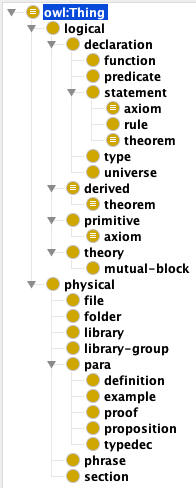
\includegraphics[width=3.5cm]{classes}\vspace*{.5em}
  \caption{ULO Classes}\label{fig:classes}\vspace*{-3em}
\end{wrapfigure}
Note that while we hold the distinction of these five classes to be universal, concrete logics may not always distinguish them syntactically.
For example, HOL identifies functions and predicates, but the extractor can indicate whether a declaration's return type is the distinguished type of booleans.
Similarly, Curry-Howard-based systems identity predicates and types as well as statements and objects, which an extractor may choose to separate.

% The semantically meaningful sorts come in three pairs each containing a type-like sort $s$ and an object-like sort $t$.
% Intuitively, individuals $i$ and $j$ of sorts $s$ and $t$ occur together in some kind of is-a or is-instance-of relation such as a typing judgment $j:i$.


% \ind{type} and \ind{function}: These are the typical sorts of most objects.
%  In first-order logic, they correspond to sorts and function symbols.
%  In type theories, they correspond to type and function symbols.

%  FR: It's difficult to come up with good names for these. So I've introduced macros for now.
%  predicate used to be called 'proposition' but that is used elsewhere as a kind of theorem
%
%\truthType and \truthObject\ednote{these names are open for discussion, see source code}: In the Curry-Howard representation, these are special cases of \ind{type} and \ind{function}, but for relating and querying libraries, it is valuable to distinguish them, and even for systems that internally use the Curry-Howard representation, it is desirable to tease them apart.  $i$ is a \truthType if it is/returns a boolean, formula, judgment etc. (regardless of its truth value), and $i$ is a \truthObject if it is/returns anything that establishes the truth of such a formula (e.g.\ axiom, theorem, proof rule).
%
%We use the \ind{rule} class to indicate that a statement can be or is interpreted as a simplification or rewrite rule, Coq has more roles like these, e.g.: \ind{coercion} (to automatically cast a value from a type to another type), \ind{hint} (to automatically try to apply it when doing blind proof search), \ind{instance} of a type-class, to be used during user-guided proof search when guessing the parameters marked to be guessed using type-classes, \ind{morphism} to be used by setoid-rewriting tactics, etc.

Orthogonally to the above, we distinguish declarations by their definition status: \ind{primitive}{\isabelle\coq} if it introduces a new concept without a definition such as an urelement or an axiom; and \ind{derived}{\isabelle\coq} if it can be seen as an abbreviation for an existing concept like a defined operator or a theorem.
For example, intersecting the classes \truthObject and \ind{derived}, we capture all theorems.

While the primitive-derived distinction is clear-cut for definition-based systems like Coq, it is trickier for axiom-based systems like Isabelle: an Isabelle definition actually consists of a primitive concept with a defining axioms for it.
For that purpose, we introduce the \ind{defines} property in \S\ref{sec:objprops}.
%\ednote{CSC: possible alternative names: \ind{defined} and \ind{declared}. Question: is it worth distinguish between defined implicitly, e.g. as the unique object that has some property vs explicitly, by describing the object?}
  
\paragraph{Physical Role}
The physical classes describe an individual's role in the physical organization of a library.
This includes for an individual $i$:
\begin{compactitem}
 \item \ind{section}{\isabelle} if $i$ is an informal grouping inside a file (chapter, paragraph etc.)
 \item \ind{file}{\coq} if $i$ is a file
 \item \ind{folder}{\coq} if $i$ is a grouping level above source files inside a library, e.g., a folder, sub-package, namespace, or session
 \item \ind{library}{\coq} if $i$ is a library. Libraries have logical URIs and serve as the root objects containing all other individuals.
 A library is typically maintained and distributed as a whole, e.g., via a GitHub repository.
 A library has a logical URI and the URIs of individuals are typically formed relative to it.
 \item \ind{library-group}{\coq} if $i$ is a group of libraries, e.g., a GitHub group.
\end{compactitem}

\noindent In addition we define some classes for the lowest organizational level, called \emph{logical paragraphs}.
These are inspired by definition--example--theorem--proof seen in informal mathematics and often correspond to {\LaTeX} environments.
In formal libraries, the individuals of these classes may be the same as the ones for the logical classes or different ones.
For example, a document-oriented system like Isabelle could assign a physical identifier to a paragraph and a different logical one to the formal theorem inside it.
These identifiers could then have classes \ind{proposition} and \truthObject respectively. %\ednote{FR: This is a good example of our names still being unintuitive.}
A purely formal system could omit the physical class or add it to the logical identifier, e.g., to mark a logical definition as an \ind{example}{\coq} or \ind{counter-example}.
Some of these, in particular, theorems given informal classes like ``Lemma'' or ``Hauptsatz'', a string which can be specified by the \ind{paratype} relation (see below).
 
%We use the class \ind{phrase} for intra-sentential fragments of in mathematical text and formulae, these include symbols, declarations, and quantifications.

\subsubsection{Properties}\label{sec:objprops}

All properties are binary predicates whose first argument is an individual.
The second argument can be an individual (\textbf{object property}) or a value (\textbf{data property}).
Unless mentioned otherwise, we allow the same property to be used multiple times for the same individual.

The two kinds are often treated differently.
For example, for visualization as a graph, we can make individuals nodes (using different colors, shapes etc. depending on which classes a node has) and object properties edges (using different colors, shapes, etc. for different properties).
The data properties on the other hand would be collected into a key-value list and visualized at the node.
Another important difference is during querying: object properties are relations between individuals and thus admit relational algebra such as union and intersection or symmetric and transitive closure.
Data properties on the other hand are usually used with filters that select all individuals with certain value properties.

\paragraph{Library Structure}
Individuals naturally form a forest consisting e.g., of (from roots to leafs) library groups, libraries, folders, files, section, modules, groups of mutual recursive objects, constants.
Moreover, the dependency relation between individuals (in particular between the leaves of the forest) defines an orthogonal structure.

$\ind{specifies}(i,j)${\isabelle\coq} expresses that $j$ is a child of $i$ in the forest structure.
Thus, taking the transitive closure of \ind{specifies} starting with a library, yields all individuals declared in a library.

$\ind{uses}(i,j)${\isabelle\coq} expresses that $j$ was used to check $i$, where $j$ may include extra-logical individuals such as tactics, rules, notations.
A very frequent case is for $j$ to be an occurrence of a logical individual (e.g. a constant or a theorem). The case of occurrences leads to the question about what information can be attached to an occurrence. Examples could be: the number of repetitions of the occurrence; whether the occurrence of a constant induces a dependency on the type only, or on the actual definition as well; where the occurrence is located (e.g. in the statement vs proof, in the type vs body or in more specific positions, like as the head symbol of the conclusion, see~\cite{AGSTZ:ContMathSearchWhelp04} for a set of descriptions of positions that is useful for searching up to instantiation). For now we decided to avoid to specify occurrences in the ontology, for the lack of a clear understanding of what properties will really be useful for applications. Integrating the ULO ontology with occurrences is left for future work towards ULO 1.0.

\paragraph{Semantic Relations between Declarations}
Relational representations treat individuals as black boxes.
But sometimes it is helpful to expose a little more detail about the internal structure of a declaration.
For that we define the following properties:
\begin{compactitem}
 \item $\ind{defines}(i,j)$ is used to relate a declaration $j$ to its definition $i$ if the two have different identifiers, e.g., because they occur in different places in the source file, or because $i$ is a defining axiom for a constant $j$.
 \item $\ind{justifies}(i,j)${\isabelle} relates any kind of argument $i$ to the thesis $j$ it supports. The most important example is relating a proof to its theorem statement if the two have different identifiers.
 \item $\ind{instance-of}(i,j)${\isabelle\coq} relates a structuring declaration $j$ to the theory-like entity $i$ that realizes, e.g., a module to its module type, an instance to its (type) class, a model to its theory, or an implementation to its specification.
 \item $\ind{generated-by}(i,j)$ expresses that $i$ was generated by $j$, e.g., the user may define an inductive type $j$ and the systems automatically generated an induction schema $i$.
 \item $\ind{inductive-on}(i,j)${\isabelle} expresses that $i$ is defined/proved by induction on the type $j$.
\end{compactitem}

\paragraph{Informal Cross-References}
First we define some self-explanatory cross-references that are typically (but not necessarily) used to link individuals within a library. These include \ind{same-as}, \ind{similar-to}, \ind{alternative-for}, \ind{see-also}, \ind{generalizes}, and \ind{antonym-of}.

Second we define some cross-references that are typically used to link a knowledge item in a library to the outside.
Of particular relevance are:
\begin{compactitem}
 \item $\ind{formalizes}(i,j)$ indicates that $j$ is an object in the informal realm, e.g., a theorem in an article, that is formalized/implemented by $i$.
 \item $\ind{aligned-with}(i,j)$ indicates that $i$ and $j$ formalize/implement the same mathematical concept (but possibly in different ways).
% \item \ind{inspired-by} and  are self-explanatory.
\end{compactitem}

\paragraph{Data Properties}
All properties so far were object properties.
Data properties are mostly used to attach metadata to an individual.
We do not introduce new names for the general-purpose metadata properties that have already been standardized in the Dublin Core such as
\verb|dcterms:creator|,
\verb|dcterms:title|,
\verb|dcterms:contributor|,
\verb|dcterms:description|,
\verb|dcterms:date|,
\verb|dcterms:isVersionOf|,
\verb|dcterms:source|,
\verb|dcterms:license|.
But we define some new data properties that are of particular interest for math libraries:
\begin{compactitem}
 \item $\ind{name}(i,v)${\isabelle\coq} attributes a string $v$ to a declaration that expresses the (user-provided) name as which it occurs in formulas.
 This is necessary in case an individual generated URI is very different from the name visible to users, e.g., if the URI is generated from an internal identifier or if the name uses characters that are illegal in URIs.
 \item $\ind{sourceref}(i,v)${\isabelle\coq} expresses that $v$ is the URI of the physical location (e.g., file, line, column in terms of UTF-8 or UTF-16 characters) of the source code that introduced $i$.
 \item $\ind{docref}(i,v)${\coq} expresses that $v$ is the URI reference to a place where $f$ is documented (usually in some read-only rich text format).
 \item $\ind{check-time}(i,v)${\isabelle} expresses that $v$ is the time (a natural number giving a time in milliseconds) it took to check the declaration that introduced $i$.
 \item $\ind{external-size}(i,v)${\isabelle} expresses that $v$ measures the source code of $i$ (similar to positions above).
 \item $\ind{internal-size}(i,v)${\coq} expresses that $v$ is the number of bytes in the internal representation of $i$ including inferred objects and generated proofs.
 \item $\ind{paratype}(i,v)${\isabelle} gives the ``type'' of a logical paragraph, i.e. something like ``Lemma'',  ``Conjecture'', \ldots. This is currently a string, but will become a finite enumeration eventually.
\end{compactitem}
Locations, sizes, and times may be approximate

\paragraph{Organizational Status}
Finally, we define a few (not mutually exclusive) classes that library management--related information such as being experimental or deprecated.
Many of these are known from software management in general.
The unary properties are realized as data properties, where the object is an explanatory string, the binary relations as object properties. 
An important logic-specific class is \ind{automatically-proved} --- it applies to any theorem, proof step, or similar that was discharged automatically (rather than by an interactive proof).

%%% Local Variables:
%%% mode: latex
%%% mode: visual-line
%%% fill-column: 5000
%%% TeX-master: "report"
%%% End:

%  LocalWords:  textbf organizational ednote swMATH irrelavant mathbb newcommand xspace mathrm emph formalized wrapfigure vspace includegraphics setoid-rewriting sec:objprops organization compactitem visualization visualized subsubsection noindent i,j dcterms:creator dcterms:title dcterms:contributor dcterms:description dcterms:date dcterms:isVersionOf dcterms:source dcterms:license i,v sourceref docref realized
